%-----------------------------------------------------------------------------
%
%               Template for sigplanconf LaTeX Class
%
% Name:         sigplanconf-template.tex
%
% Purpose:      A template for sigplanconf.cls, which is a LaTeX 2e class
%               file for SIGPLAN conference proceedings.
%
% Guide:        Refer to "Author's Guide to the ACM SIGPLAN Class,"
%               sigplanconf-guide.pdf
%
% Author:       Paul C. Anagnostopoulos
%               Windfall Software
%               978 371-2316
%               paul@windfall.com
%
% Created:      15 February 2005
%
%-----------------------------------------------------------------------------


\documentclass[preprint,nocopyrightspace,10pt]{sigplanconf}

% The following \documentclass options may be useful:
%
% 10pt          To set in 10-point type instead of 9-point.
% 11pt          To set in 11-point type instead of 9-point.
% authoryear    To obtain author/year citation style instead of numeric.

\usepackage{rotating}
\usepackage{algpseudocode}
\usepackage{algorithm}% http://ctan.org/pkg/algorithms
\usepackage{algpseudocode}% http://ctan.org/pkg/algorithmicx
%\usepackage{syntax}

\usepackage{amsmath}
\usepackage{graphicx}
\usepackage{xspace}
\usepackage[
		pdfauthor={Peizhao Ou and Brian Demsky},
		pdfkeywords={concurrent data structures, specification language, model
		checking},
]{hyperref}
\usepackage{amssymb}

\usepackage{listings}
\usepackage{color}
\usepackage{textcomp}
\definecolor{listinggray}{gray}{0.9}
\definecolor{lbcolor}{rgb}{0.9,0.9,0.9}
\lstset{
	% backgroundcolor=\color{lbcolor},
	% rulecolor=,
	% aboveskip={1.5\baselineskip},
	% extendedchars=true,
	tabsize=3,
	language=C++,
	basicstyle=\ttfamily\scriptsize,
	upquote=true,
	columns=fixed,
	showstringspaces=false,
	breaklines=true,
	prebreak = \raisebox{0ex}[0ex][0ex]{\ensuremath{\hookleftarrow}},
	% frame=single,
	showtabs=false,
	showspaces=false,
	showstringspaces=false,
	identifierstyle=\ttfamily,
	keywordstyle=\color[rgb]{0,0,1},
	commentstyle=\color[rgb]{0.133,0.545,0.133},
	stringstyle=\color[rgb]{0.627,0.126,0.941},
	numbers=left,
	numberstyle=\tiny,
	numbersep=8pt,
	escapeinside={/*@}{@*/}
}

\usepackage{algpseudocode}

%% Not used yet
% \usepackage{times}
% \usepackage{latexsym}
% \usepackage{amsfonts}
% \usepackage{amsthm}
% \usepackage{txfonts}
% \usepackage{url}
% \usepackage{subfigure}

% \usepackage{bbm}
% \usepackage{stfloats}

\newcommand{\code}[1]{\text{\tt #1}}
\newcommand{\mypara}[1]{\noindent {#1}}
\newcommand{\etal}{\textit{et al}.\xspace}
\newcommand{\cdschecker}[0]{\textsc{CDSChecker}\xspace}
\newcommand{\TOOL}[0]{\textsc{SCFence}\xspace}

\newcommand{\TODO}[0]{\textbf{TODO}\xspace}
\newcommand{\todo}[1]{{\bf [[#1]]}}
%\newcommand{\todo}[1]{}
\newcommand{\comment}[1]{}
\newcommand{\tuple}[1]{\ensuremath \langle #1 \rangle}
\newcommand{\rf}{\reltext{rf}}
\newcommand{\reltext}[1]{\textit{#1}}


\begin{document}

\conferenceinfo{ISSTA '14}{date, City.} 
\copyrightyear{2014} 
\copyrightdata{[to be supplied]} 

\sloppy

\title{\TOOL: Automatic Inference of Memory Order Parameters to Obtain SC Behaviors under C/C++11}

\authorinfo{Peizhao Ou and Brian Demsky}{University of California, Irvine}{\{peizhaoo,bdemsky\}@uci.edu}

\maketitle

\begin{abstract}
\input{abstract}
\end{abstract}

\section{Introduction}\label{sec:introduction}

\section{Motivating Example}
\label{sec:example}

\section{Technical}\label{sec:technical}

\subsection{Inference Rules}
Previous work takes advantage of model-checking approach to check whether a
specific C/C++11 trace is sequentially consistent. By building up edges
(\textit{sb}, \textit{rf} and \textit{sc} by implication rules) between atomic
operations, it judges whether the trace is SC by whether there exists a cycle in
that graph. Besides, when it finds a non-SC trace, it has a sorting algorithm
that generates an SC-like trace and exposes which reads-from edge that causes a
cycle.

Under the C/C++11 memory model, inferring the ordering parameters to obtain SC
behaviors is essentially a searching problem. In the absence of consume
operations, memory order parameters for atomic operations can be only one of the
following: \textit{memory\_order\_relaxed}, \textit{memory\_order\_release},
\textit{memory\_order\_acquire}, \textit{memory\_order\_acq\_rel} and
\textit{memory\_order\_seq\_cst}. By enumerating all possible memory order
parameters, we can guarantee that we can find out all the possible inference of
parameters that ensure SC behaviors for a specific test case. However, this
naive approach obviously leads to an exponential searching space.

Actually, when we have a non-SC execution, we have some knowledge availabe
reflecting where the problem may lie. Consider we start from the case where all
memory order parameters are \textit{memory\_order\_relaxed}. Whenever the
model-checking approach finds out a cycle in a specific execution, we have to
infer some stronger memory orders to eliminate the cycle. What causes the cycle
to happen leads to the non-SC trace. We propose a search-based approach combined
with cycle patterns and their fixes to reduce searching space.

In Figure~\ref{fig:fence_implications} , we show a number of universal patterns
that can exist in cycles. We explain how we should fix those cycle patterns
respectivelys the following.

\mypara{\bf Circular \textit{sb} $\cup$ \textit{rf}:} If a cycle is composed of
edges which are the union of \textit{sb} \& \textit{rf}, a universal fix is to
make all but one of the atomic operation \textit{happen-before} the next atomic
operation in that cycle. It is worth noting that imposing
\textit{happens-before} to ajacent nodes is not limited to imposing
release/acquire pairs to store/load operations involed in the cycle. Instead,
any possible paths composed with the union of \textit{sb} $\cup$ \textit{rf}
between the two nodes can be strengthened.

\mypara{\bf Old value read \RNum{1}:} When we sort the trace into an SC-like
ordering, we may encounter the case where a load reads from some old store
and those three operations can be connected via at least one path composed on
the union of \textit{sb} $\cup$ \textit{rf}. A universal fix for this pattern is
to impose \textit{happens-before} between the two stores and
\textit{happens-before} between the recent store and the load at the same time.

\mypara{\bf Old value read \RNum{2}:} Similar to the previous pattern, we see a
load read from an old store. However, the difference is that we do not have a
union of \textit{sb} $\cup$ \textit{rf} between the two stores and between the
recent store and the load at the same time. To fix this problem, we need to
impose the following: 1) the old store \textit{modification-order} before the
recent store (weaker than \textit{sc} or \textit{hb}); 2) the recent store
\textit{sc} before the load or the \textit{happens-before} the load.


\mypara{\bf Future value read:} Unlike reading an old value in the trace,
another possible pattern is reading a future value. To fix this pattern, we can
do the following: 1) impose \textit{happens-before} from the store to the load;
2) impose \textit{sc} from the load to the store.


Figure~\ref{fig:algorithm} shows the core searching algorithm for all possible
parameters.

\begin{figure}[!ht]
\centering
\begin{tabular}{c}
\multicolumn{1}{c}{Circular \textit{sb} \& \textit{rf}}\\
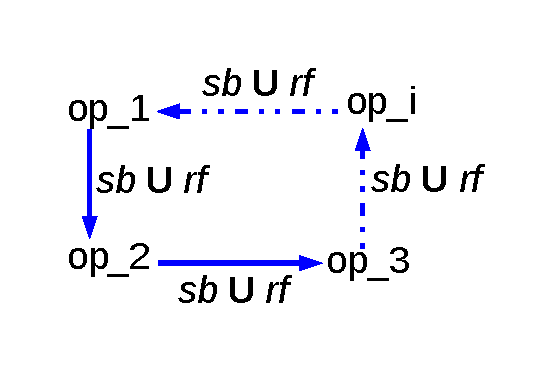
\includegraphics[scale=.45]{figures/circular_sb_rf}\\
\multicolumn{1}{c}{Old Value Read \RNum{1}}\\
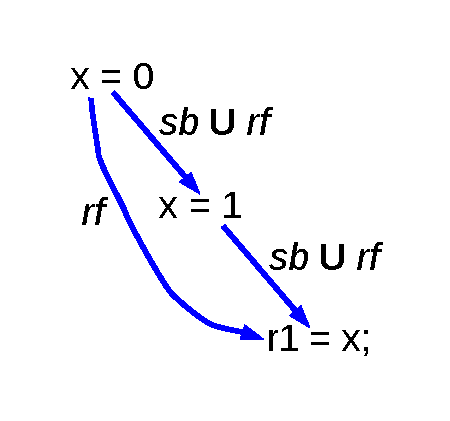
\includegraphics[scale=.45]{figures/old_val_sync}\\
\multicolumn{1}{c}{Old Value Read \RNum{2}}\\
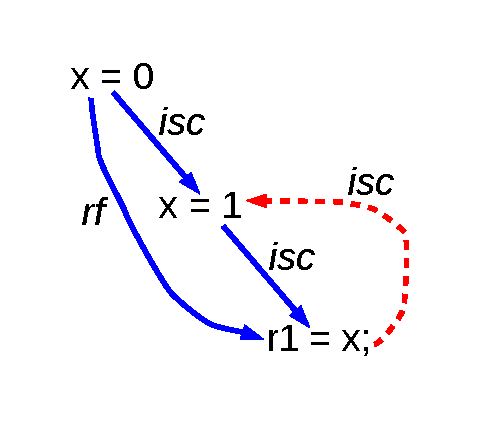
\includegraphics[scale=.45]{figures/old_val_isc}\\
\multicolumn{1}{c}{Future Value Read}\\
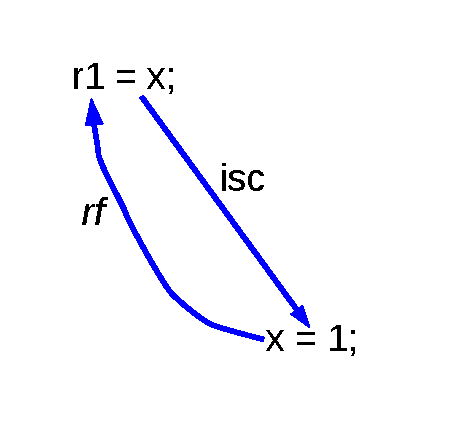
\includegraphics[scale=.45]{figures/future_val_isc}\\
\end{tabular}
\caption{\label{fig:fence_implications}Cycle Patterns for Non-SC Behaviors}
\end{figure}


\begin{figure}[!htbp]
\begin{algorithmic}[1]
\Function{InferParams}{}
\State candidates := \{\}
\State candidate $c1$ := replace all wildcards with \textit{relaxed}
\State candidates += $c1$
\State results := \{\}
\While{candidates is not empty}
\State Candidate $c$ := candidates.pop()
\State Model-check with $c$ and yield a cycle $l$
\If{$l$ == NULL}
\State results += $c$
\Else
\State \Call {StrengthenParam}{$l$, $c$, candidates}
\EndIf
\EndWhile
\State \Return{results}
\EndFunction

\Procedure{StrengthenParam}{c, p, candidates}
\While{$\exists$ a pattern $p$ in cycle $c$}
\State possible\_fixes := strengthen $c$ by pattern $p$
\State candidates += possible\_fixes 
\EndWhile
\EndProcedure

\end{algorithmic}
\caption{\label{fig:algorithm}Algorithm for Searching All Possible Parameters}
\end{figure}


\section{Evaluation}\label{sec:evaluation}

\section{\label{sec:related}Related Work}
SC~\cite{scmemorymodel}



\section{Conclusion\label{sec:conclusion}}




% We recommend abbrvnat bibliography style.
\bibliographystyle{abbrvnat}
\bibliography{confstrs-abbrv,paper}

\end{document}
